\documentclass[a4paper, 11pt, french]{report}
\usepackage{setspace}
\setstretch{1,15}
% \usepackage{fontspec}
% \setmainfont{Verdana}
\usepackage{newunicodechar}
\usepackage{babel}
\usepackage{graphicx}
\graphicspath{{images/}}
\usepackage{lipsum}
\renewcommand{\thesection}{\arabic{section}}
\usepackage{ulem}
\usepackage{geometry}
\geometry{hmargin=2.5cm,vmargin=3.5cm}



\begin{document}

\begin{title}

\title{
    {\Huge Le système d'achat de l'energie}\\
    \vspace{1 cm}
    {\LARGE JUILLIARD Quentin S5O6}\\
    {\LARGE COGNE Romain S5O6}\\
    \vspace{2.5 cm}
    {
\includegraphics[width=90mm, height=50mm]{logo_univ}}\\
    \vspace{2.5 cm}
    {\Large Monsieur BOISSON, INFO0503 / Département Informatique}\\
    \vspace{1 cm}
    {\date{\Large Dimanche 11 décembre 2022}}}
\end{title}

\maketitle
\tableofcontents
\clearpage


\pagenumbering{arabic}

\section{Introduction}


\newpage

\subsection{Relation entre Revendeur et Tare}
\newpage

\subsection{Relation entre Tare et Marché de Gros}
Le Marché de Gros et les TAREs communique entre eux à l'aide du communication UDP. Les informations qui transitent dans les requêtes sont des éléments de type SuiviCommande qui intègrent les variables de type "Energie". Voici à quoi ressemble un échange :

\begin{figure}[h]
    \centering
    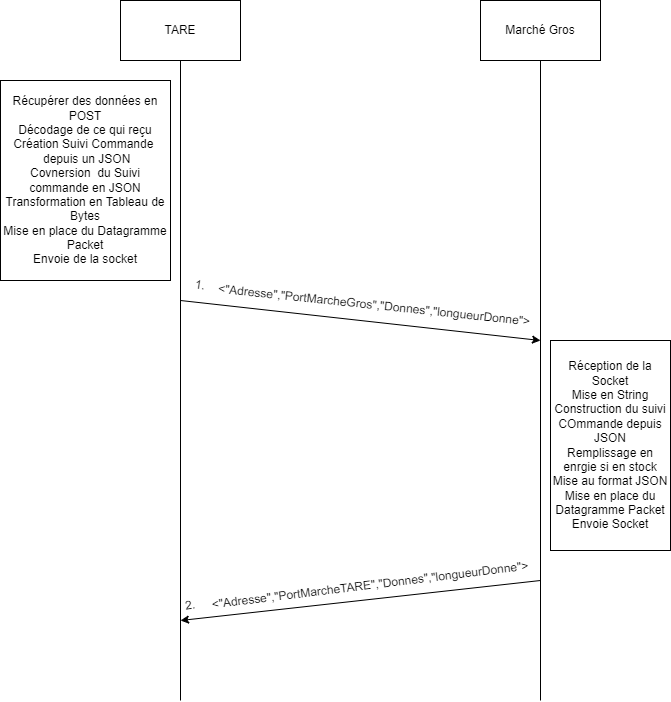
\includegraphics[width=140mm, height=120mm]{images/TAREMG.png}
    \caption{Modélisation de la relation entre Marché de Gros et PONE}
    \label{img:mesh19}
\end{figure}
\newpage

\subsection{Relation entre Marché de Gros et PONE}
Il existe une relation entre le Marché de Gros et le (ou les) PONE. Cette relation est unidirectionnel en User Datagramme Packet ( UDP ), nous envoyons des datagrammes packets du Pone contenant une énergie qui est caractérisée par :
\\
\begin{itemize}
    \item Un type d'energie,
    \item Une quantité envoyé,
    \item Un mode d'extraction,
    \item Un prix unitaire,
    \item Un numéro de lot
    \\
\end{itemize}
 Cette énergie est donc envoyée vers les marché de gros sans vérification d'aquisition car l'UDP est un protocole de transite d'informations sur internet qui n'est pas en capacité de garantir la bonne récéption des informations chez le client.
\begin{figure}[h]
    \centering
    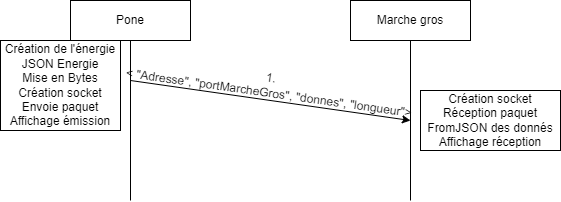
\includegraphics[width=120mm, height=45mm]{images/PONEMG.png}
    \caption{Modélisation de la relation entre Marché de Gros et PONE}
    \label{img:mesh16}
\end{figure}


\subsection{Role de l'AMI}
Dans ce réseau l'AMI ne communique uniquement avec le marché de gros en TCP. Il a pour rôle de vérifier le prix des énergies fournis par les PONE ainsi que de valider la vente avec les TAREs. De plus, l'ensemble des échanges sont sécurisés par un chiffrement RSA pour les crypter. 

Cependant l'AMI doit également certifier, signer les énergies à la sortie de leur production, on parle alors de CeRtificAt D'Origine (ou CRADO). Il doit également certifier, signer les achats, on parle alors de CeRtificAt d'aCHAt (ou CRACHA).
\newpage

\section{Diagramme}

\newpage

\subsection{Architecture Echange}
\newpage

\section{Les différentes relations}
\newpage

\subsection{Realtion HTTP}
\newpage

\subsection{Relation UDP}
\newpage

\subsection{Relation TCP}
\newpage

\subsection{Relation PHP}
\newpage

\section{Sénario}
\newpage

\subsection{Scénario A}

\newpage


\subsection{Scénario B}
\newpage

\subsection{Scénario C}
\newpage

\subsection{Scénario D}
\newpage

\subsection{Scénario A2}
\newpage

\section{Conclusion}
\newpage


\end{document}
